\chapter{評価}
\label{chap:eval}
ランサムウェアによる暗号化からデータを保護する性能と,提案手法稼働時のオーバーヘッドを評価した.
評価はすべて\tabref{tab:experiment-machine-kashiwa}に示す物理マシン上で行った.
\begin{table}[t]
  \caption{Environment of the physical machine used for the evaluation.}
  \label{tab:experiment-machine-kashiwa}
  \hbox to\hsize{\hfil
    \begin{tabular}{l|lll}
      \hline \hline
      OS       & Ubuntu 22.04.4 LTS                                  \\
      ファイルシステム & ext4                                                \\
      カーネル     & 6.3.0-060300-generic                                \\
      CPU      & \scriptsize{Intel Xeon Silver 4314 @ 2.400GHZ × 64} \\
      RAM      & 512GiB                                              \\ \hline
    \end{tabular}\hfil}
\end{table}

\section{データ保護性能の評価}
\subsection{実験シナリオ}
指定されたパスのファイルを\texttt{read}し,OpenSSL内の関数で暗号化したのち新規ファイルに\texttt{write}するプログラムをC言語で実装した.
暗号化方式はAES256を使用し,鍵長とIV長はそれぞれ32Bと16Bとした.\texttt{read}などの処理は4096Bのバッファに対して行うようにした.
このプログラムをこれ以降「\textbf{暗号化プログラム}」と称する.

OpenSSLが提供するコマンドを使用して,指定したバイト長の擬似乱数を含むファイルを生成する.
そして生成したファイルに対して以下の手続きを行う.
\begin{enumerate}
  \item 実装した提案手法を実行する.
  \item 暗号化プログラムでファイルを暗号化する.
  \item 元のファイルと,Data Shelter内に作成されたファイルを用いて評価を行う.
\end{enumerate}
% 暗号化の対象となるファイルを「\textbf{元ファイル}」
Data Shelter内に作成されるファイルを「\textbf{退避ファイル}」と呼ぶ.

この実験におけるデータ保護性能の評価指標として,\textbf{一致率}を定義した.
一致率は,退避ファイルと元ファイルがどの程度一致しているかを表す指標である.
元ファイルと退避ファイルのデータをバイト値の配列とみなし,先頭から配列の値を調べて一致している個数を数え,
その個数を元ファイルのバイトサイズで割ると一致率が求められる.
元ファイルが\texttt{[1, 2, 3, 4, 5]},退避ファイルが\texttt{[1, 2, 4]}の場合,先頭の1と2が一致しているので
この時の一致率は$\frac{2}{5}=0.4$である.

\subsection{予備実験の結果}
\label{subsec:preliminary-result}
先行研究\cite{css2024}で示した実装をによる提案手法の一致率を予備実験で評価した.
結果を\figref{fig:seq-vs-par-exp}および\figref{fig:seq-vs-par-inc}に示す.
Evacuation Moduleが実行する3つの処理Read,Decode,Writeのそれぞれの処理時間の分布を\figref{fig:elapsed-time}に示す.
\begin{figure}[h]
  \centering
  \begin{subfigure}[b]{0.48\columnwidth}
    \centering
    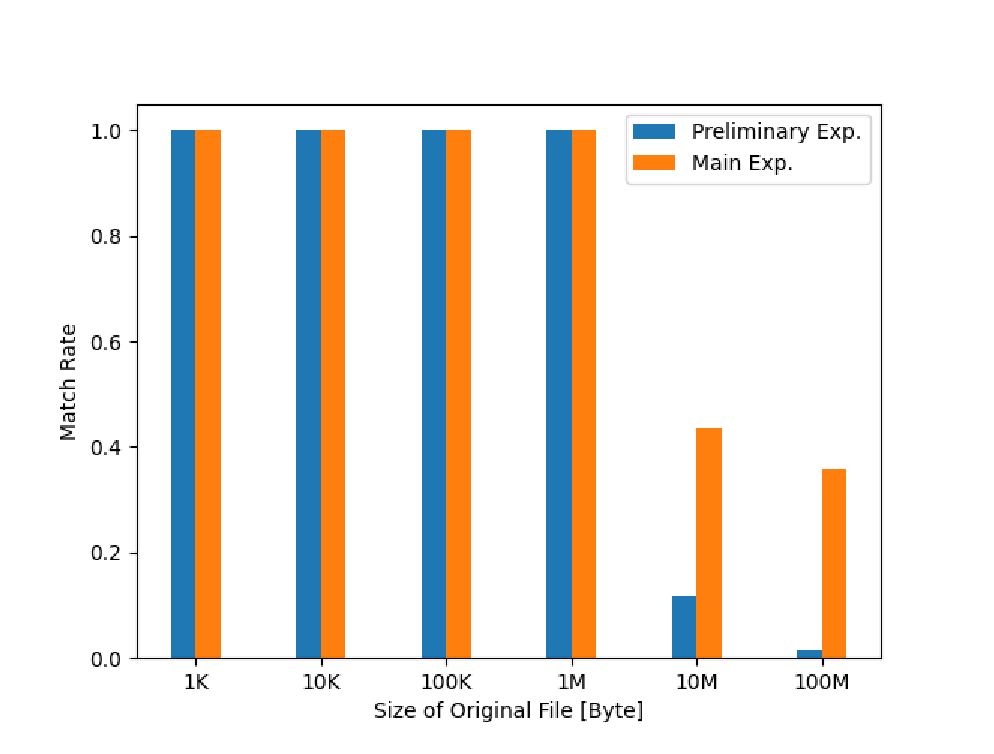
\includegraphics[width=\columnwidth]{doc/img/eval/seqential_vs_parallel_match_p4_exp.eps}
    % \caption{Match rates by original file size. The horizontal axis is presented on a common logarithmic scale,
    % comparing results from the preliminary and main experiments.}
    \caption{Match rates by original file size of 1KB, 10KB, $\ldots$, 100MB.}
    \label{fig:seq-vs-par-exp}
  \end{subfigure}
  \hspace{0.02\columnwidth}
  \begin{subfigure}[b]{0.48\columnwidth}
    \centering
    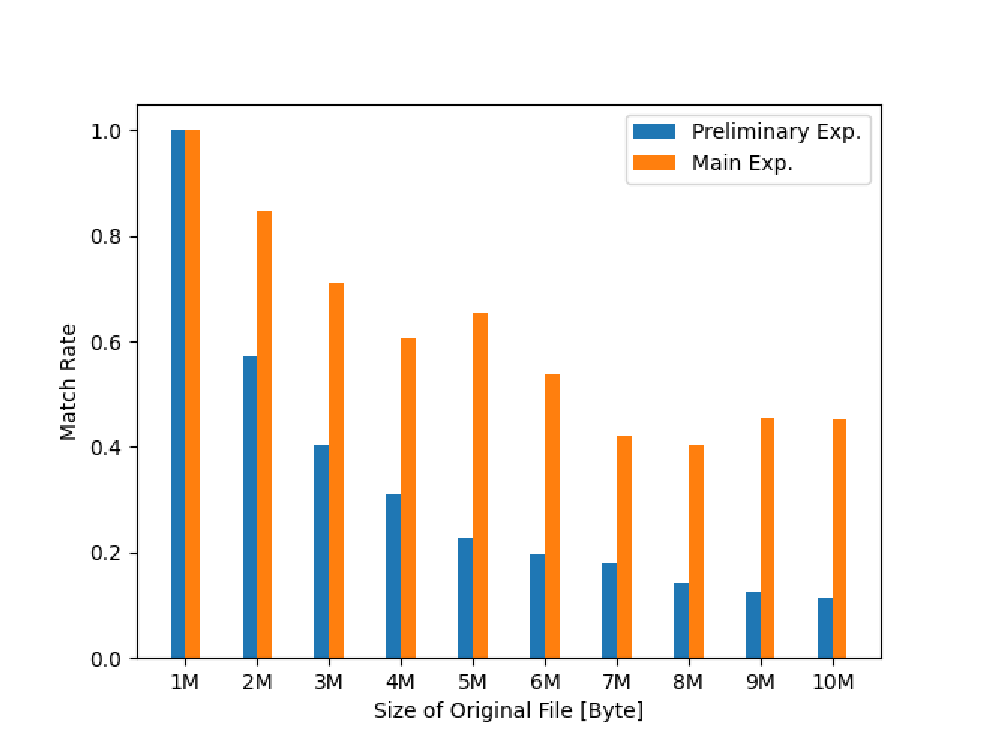
\includegraphics[width=\columnwidth]{doc/img/eval/seqential_vs_parallel_match_p4_inc.eps}
    % \caption{Match rates by original file size,
    % comparing results from the preliminary and main experiments.}
    \caption{Match rates by original file size of 1MB, 2MB, $\ldots$, 10MB.}
    \label{fig:seq-vs-par-inc}
  \end{subfigure}
  \caption{Match rates by original file size, comparing results from the preliminary and main experiments.
    The horizontal axis in the left figure uses a common logarithmic scale.}
\end{figure}

\begin{figure}[t]
  \begin{center}
    \includegraphics[width=\columnwidth]{doc/img/eval/hakohige_sequential.eps}
  \end{center}
  \caption{Boxplot of processing times for the three operations in the Evacuation Module: Read, Decode, and Write.
    Entries with processing times exceeding 1000 µs were excluded; only 2 out of 976 total entries were removed.}
  \label{fig:elapsed-time}
\end{figure}

\subsection{元ファイルのサイズに対する一致率の変化}
本稿では先行研究 \cite{css2024} と同様に,
1KB,10KB,$\ldots$,100MBのサイズの元ファイルに対して実験を行い,一致率を計算した.
Decode処理の並列度は4に,リングバッファのサイズは1MiBに設定した.
その結果を\figref{fig:seq-vs-par-exp}に示す.
また,1MBから10MBまで1MB刻みのサイズのファイルを生成し実験を行った.並列度とリングバッファの設定は同一である.
結果を\figref{fig:seq-vs-par-inc}に示す.
先行研究 \cite{css2024} で示された一致率からの向上が確認され,
高速化,すなわちEvacuation Moduleのパイプライン化とデコード処理の並列化,が保護性能の改善に寄与したことがわかった.
性能改善の程度は元ファイルのサイズが大きいほど顕著であり,100MBの元ファイルに対しては20倍以上の差が見られた.

\subsection{パラメータの変更に対する一致率の変化}
本稿で示した実装は,デコード処理の並列度($=p$)とリングバッファのサイズ($=|RB|$)をパラメータとして持つ.
2つのパラメータのうち一方を固定しもう一方を変化させて実験を行い,各パラメータが一致率に与える影響を調査した.

$p$を固定し$|RB|$を2MiBから2倍ずつ大きくした時の一致率の変化を\figref{fig:buf-capability}に示す.
$|RB|$より小さいファイルは完全に保護することができるが,$|RB|$より大きいファイルに対しては各$|RB|$間で類似した傾向で保護性能が低下する.
\begin{figure}[tb]
  \centering
  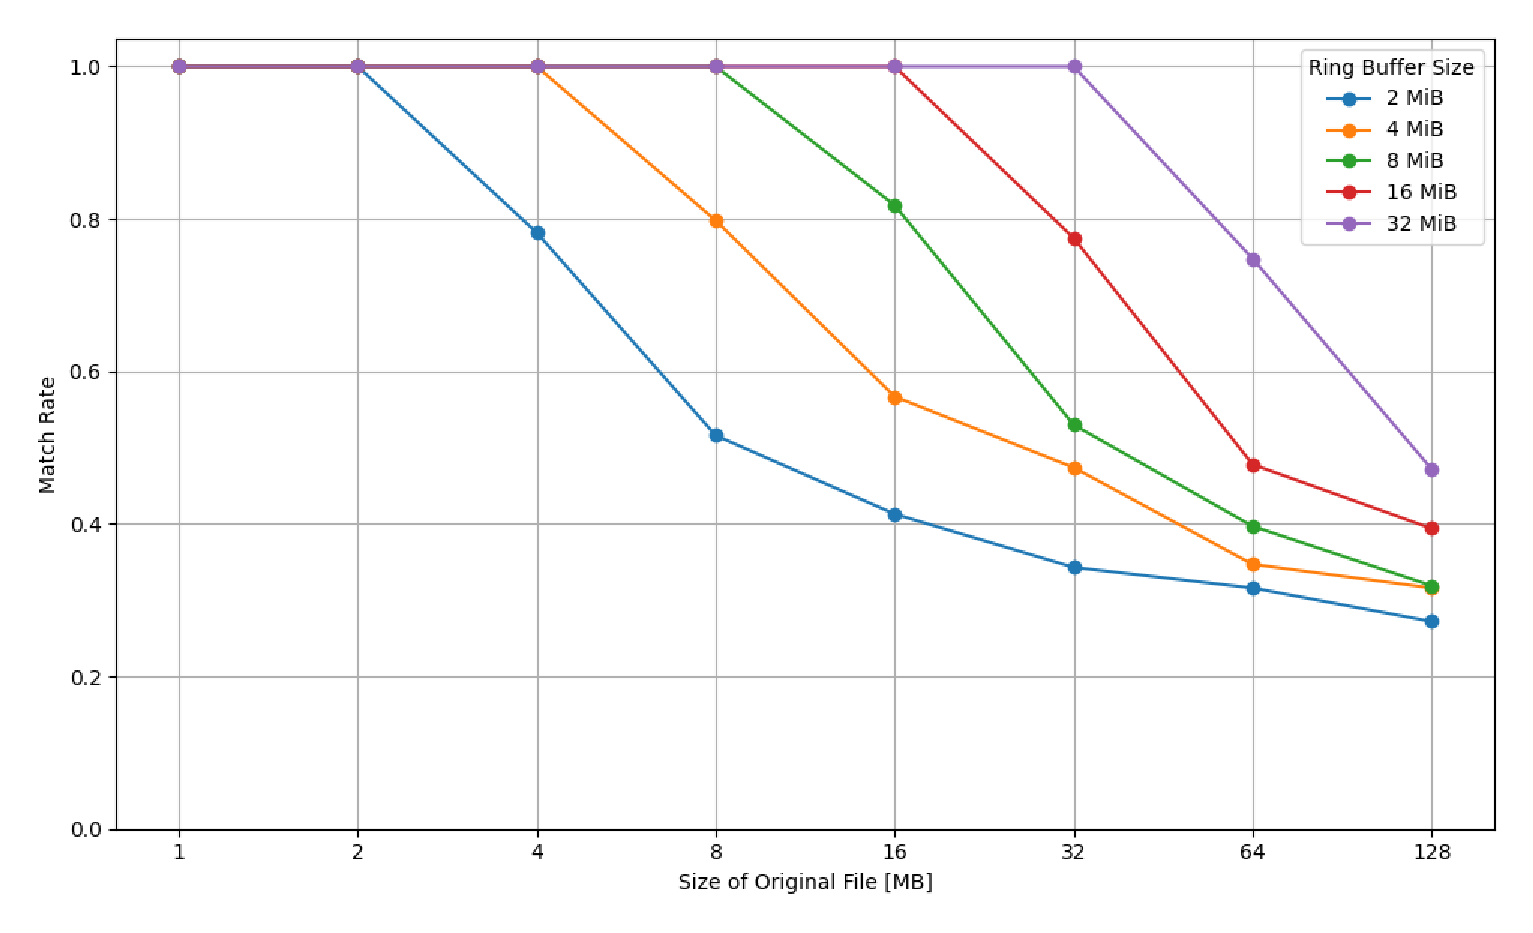
\includegraphics[width=0.9\columnwidth]{doc/img/eval/buf_capability_seek.eps}
  \caption{Variation of match rate by file size for different ring buffer sizes. The horizontal axis uses a logarithmic scale (base 2).}
  \label{fig:buf-capability}
\end{figure}

$|RB|$を固定し$p$を様々な値に設定した時の一致率の変化を\figref{fig:diff-parallelism}に示す.
$p$を増加させるほど,完全に保護可能なファイルのサイズは増加する傾向が見られる.
元ファイルのサイズの増加に対して一致率は単調に減少すると期待されるがそうなっておらず,
並列処理スレッドのスケジューリングの状況に依存して性能が変化する可能性がある.
\begin{figure}[tb]
  \centering
  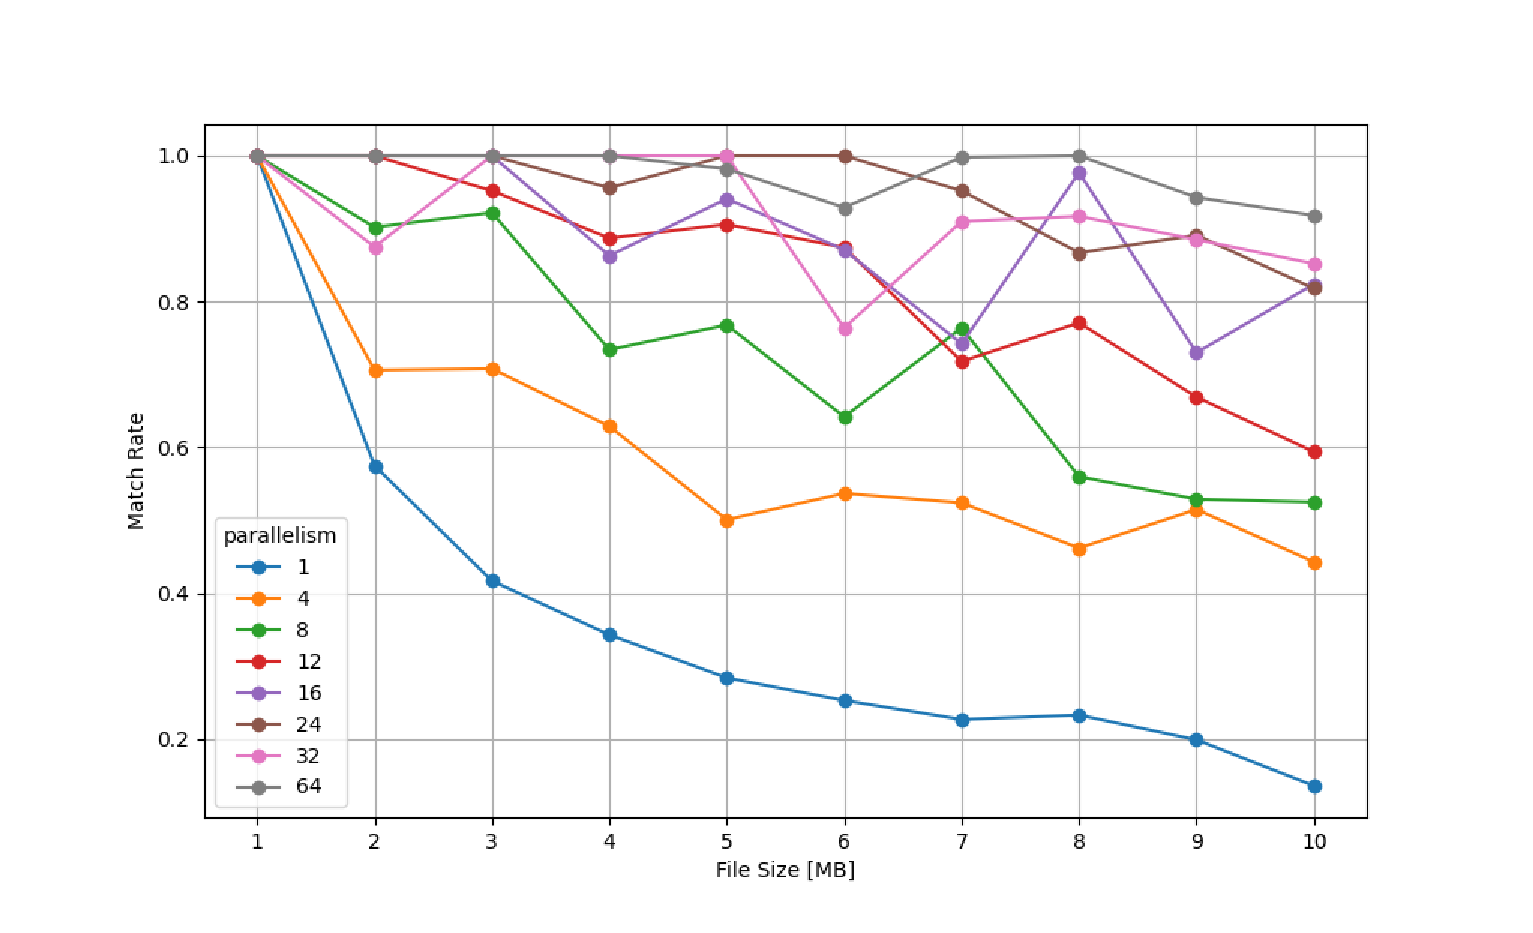
\includegraphics[width=\columnwidth]{doc/img/eval/match_seek_diff_parallelism.eps}
  \caption{Variation of match rate by original file size for different degrees of parallelism $p$.}
  \label{fig:diff-parallelism}
\end{figure}

パラメータ$p$を大きくすると多数のスレッドが生成されるため高いコア数が求められ,CPU使用率が増加する.
一方,$|RB|$を増やすことはカーネル空間のメモリ消費を伴うが,32MiB程度の設定は現実的であり,
計算リソースに対する保護性能の向上効果が大きいと我々は考える.
もちろん$p$と$|RB|$の両方を同時に大きくすることも可能である.

しかしながら,パラメータを調整しても100MB〜数GBオーダーの大きさのファイルを完全に保護することは現実的ではない.
頻繁に更新されないファイルならば定期的なスナップショットを利用してバックアップを確保することが望ましく,
保護したいファイルの大きさに応じて適切な戦略が異なるといえる.

\section{オーバーヘッドの評価}
\subsection{CPU使用率とI/O wait}
本稿で示す実装では,Data Shelterとして使用されているディレクトリに大量にデータの書き込みが発生する.
また,ランサムウェアが高速にファイルを暗号化する場合,Process MonitorおよびEvacuation Moduleは高い頻度で
データを処理する必要がある.
したがって提案手法はCPU使用率およびディスクI/Oにオーバーヘッドを発生させることが予想されるため,これらのメトリクスを計測した.

メトリクスの取得には\texttt{iostat}を利用した.
\texttt{iostat}はユーザ空間およびカーネル空間のCPU使用率の平均値,I/O wait率の平均値,ブロックデバイスごとのread/writeの量などを出力するコマンドである,
本研究では1秒ごとにデータを記録する設定を用いた.
汎用的なマクロベンチマークのセットであるsysbench \cite{sysbench:online} の\texttt{fileio}ベンチマークを使って
16MiBのファイルを128個生成し,暗号化プログラムによって各ファイルを暗号化することでワークロードを発生させた.
暗号化プログラムによる暗号化を開始した時点を$t = 0$とし,30秒の間\texttt{iostat}の出力を続けた.

システム全体のベースライン (A),提案手法を使用せずに暗号化を行なった場合 (B),提案手法を使用して暗号化を行なった場合 (C) の3パターンで計測を行った.
計測間のばらつきを抑えるために,計測は各パターンで5回ずつ行い平均値を計算した.

CPU使用率の推移を\figref{fig:cpu-usage}に,I/O wait率の推移を\figref{fig:iowait}に示す.
CPU使用率は1.5\%増加しており,提案手法のデータ退避処理がCPUリソースを多く消費することがわかる.
一方I/O wait率については,一時的な増加は見られるものの増加幅は最大でも0.05\%程度であり,
提案手法がディスクI/Oに与えるオーバーヘッドは非常に小さい.
全体として,提案手法ではCPUが主なボトルネックであると考えられる.

\begin{figure}[tb]
  \centering
  \includegraphics[width=0.8\columnwidth]{doc/img/eval/cpu_usage.eps}
  \caption{The transition of CPU usage.}
  \label{fig:cpu-usage}
\end{figure}

\begin{figure}[tb]
  \centering
  \includegraphics[width=0.8\columnwidth]{doc/img/eval/iowait_usage.eps}
  \caption{The transition of I/O wait.}
  \label{fig:iowait}
\end{figure}

\subsection{データ退避スループットの推定}
前節で述べたパターン(C)では提案手法による書き込みが発生するが,パターン(B)では発生しない.
したがってパターン(B)および(C)での書き込みスループットの差を取ることで,提案手法が
ファイルを退避させるスループットを推定することができる.
30秒ごとの\texttt{iostat}の出力を5回取得し,統計値を計算した.

\tabref{tab:performance_metrics}に示す結果から,本稿で示した提案手法の実装は19MB/s程度のスループットで
データを退避させることができると示唆される.
ここで,ランサムウェアがデータを暗号化するスループットを推定し,提案手法のスループットと比較する.
Huangら \cite{huang2017flashguard} が行ったランサムウェア対策の開発の事前調査を参照すると,
ランサムウェアによるファイル暗号化のスループットは1MB/sから4MB/s程度であると計算される.
\cite{huang2017flashguard}から引用したデータ,および筆者による計算結果を\tabref{tab:ransomware_performance}に示す.
したがって提案手法はランサムウェアによる暗号化よりも高速にデータを退避することができ,
ランサムウェアのプロセスが検知技術によって特定および停止されるまでの間ファイルデータを保護する性能を持つといえる.

\tabref{tab:ransomware_performance}のデータは,
本研究の実験環境(\tabref{tab:experiment-machine-kashiwa})と比較して計算資源が限られた環境で取得されたものである.
このため,ランサムウェアの暗号化スループットは,本研究の実験環境にて計測した場合,より高い数値が得られる可能性がある.
% ことに注意する必要がある.
しかし,提案手法は依然としてランサムウェアに対して十分な性能を持つと考える.
その理由は,\tabref{tab:performance_metrics}の結果が$p = 4$および$|RB| = 1$MiBの設定で得られたものであり,
仮にランサムウェアの暗号化スループットが\tabref{tab:ransomware_performance}の数値を上回る環境であっても,
提案手法のパラメータを適切に調整することでスループットの向上が可能だからである.

% \tabref{tab:performance_metrics}に示す結果より,本稿で示した提案手法の実装は約19MB/sのスループットでデータを退避できることが示された.
% 一方,Huangら\cite{huang2017flashguard}の調査に基づく計算によれば,ランサムウェアによるファイル暗号化のスループットは1MB/s ~ 4MB/s 程度である.
% これにより,提案手法はランサムウェアが起動してから検知されるまでの間に発生する暗号化に対して,ファイルデータを退避によって保護できる性能を備えているといえる.

\begin{table}[t]
  \centering
  \caption{Estimated performance metrics in MB/s.}
  \begin{tabular}{lcc}
    \hline
    Metric  & Value [MB/s] \\
    \hline
    Mean    & 18.65        \\
    Median  & 117.53       \\
    Std Dev & 825.78       \\
    \hline
  \end{tabular}
  \label{tab:performance_metrics}
\end{table}


\begin{table}[htbp]
  \centering
  \caption{Ransomware families and their encryption performance.
    The throughput column is calculated independently by the author,
    whereas the data for the other columns are cited from \cite{huang2017flashguard}.}

  \label{tab:ransomware_performance}
  \begin{tabular}{lccc}
    \hline
    Family         & Encrypted Data Size (GB) & $T$ (min) & Throughput (MB/s) \\
    \hline
    CTB-locker     & 1.9                      & 14        & 2.23              \\
    Jigsaw         & 3.2                      & 16        & 3.33              \\
    Mtobef         & 2.2                      & 16        & 2.29              \\
    Maktub         & 4.0                      & 22        & 3.03              \\
    Stampado       & 2.3                      & 27        & 1.42              \\
    Cerver         & 3.7                      & 37        & 1.67              \\
    Locky          & 4.1                      & 43        & 1.59              \\
    7ev3n          & 4.0                      & 44        & 1.52              \\
    TeslaCrypt     & 3.5                      & 44        & 1.33              \\
    HydraCrypt     & 4.1                      & 70        & 0.98              \\
    CroptoFortress & 3.9                      & 75        & 0.87              \\
    CryptoWall     & 4.0                      & 75        & 0.89              \\
    \hline
  \end{tabular}
\end{table}


